This chapter discusses the Microservice architecture. It also discusses why this architecture is being preferred over the service-orientated architecture.

The term “Microservice” was first used at a software architects workshop held in Venice in May 2011 as stated by Martin Fowler \cite{MartinFowlersite}. Participants began to realise they were using and exploring the same architectural style. It was a year later it was decided as the more appropriate name \cite{MartinFowlersite}.
As Microservices Architecture (MSA) is a relatively new architecture, there is no official industry consensus regarding the properties nor definition of MSA.

According to Sam Newman \cite{NewmanMSA} Microservices are: “small, autonomous services that work together”. Martin Fowler \cite{MartinFowlersite} continues this definition by saying “Microservices are a way of designing software applications as suites of independently deployable services”.
Microservices help break the boundaries of large applications and create smaller systems (the services) that are used to build applications as seen in figure \ref{fig:MonovMSA}.
\begin{figure}[h]
	\caption{Monolithic vs Microservices Architecture}
	\label{fig:MonovMSA}
	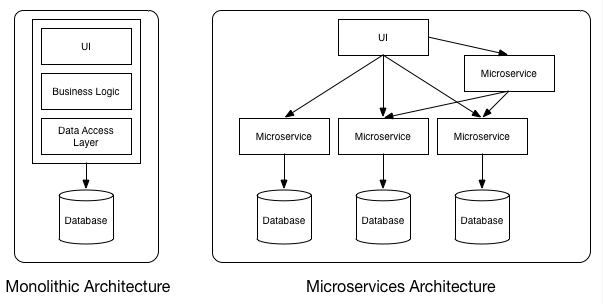
\includegraphics{MSAexample}
	\centering
\end{figure}
Tomas Cerny et al \cite{ContextUnderstandingMSA} have described Microservices as being based on three Unix ideas:
\begin{itemize}
	\item A program should fulfil only one task and do it well
	\item Programs should be able to work together
	\item Programs should use a universal interface
\end{itemize}
The implementation of MSA is open to interpretation. Though there are some defining characteristics that are commonly cited \cite{GuptaMSA} \cite{MartinFowlersite} \cite{ContextUnderstandingMSA}. Although
Zimmerman in his paper \cite{Zimmermann2017} explores the argument that the Microservice architecture itself is in fact not an Architecture but an implementation of the Service Orientated Architecture. But does state there is, currently, no consensus on the relationship between MSA and SOA.

\subsubsection{Services Are independently deployable}
Unlike traditional monolithic applications that contain several modules that may be dependent on several libraries, environment etc. Each service, within a Microservice architecture, can be deployed independently. All dependencies: database, library dependencies and execution environments such as web servers or Virtual Machine (VM) are contained within each service. This ability is what enables each service to deploy independently and be essentially autonomous as described by Gupta \cite{GuptaMSA}. Therefore, each individual service will only contain the dependencies it needs. And can be deployed for use and perform its intended function. Even if no other service is available, the deployed services will perform their intended function, barring failure: hardware, software etc.

As services can be deployed on different machines, a distributed system of services, this can help with fault tolerance. If only a single service is on a machine that fails for whatever reason. Then it will not affect the rest of the services increasing the fault tolerance of the system or program.

Each of the independent services deployed combine to make the intended application(s). Such as an E-Commerce web application, news web application etc.

\subsubsection{Services are built around business capabilities}
The more recognised model of focusing on the technology layer of applications results in creating different development teams for: UI, server-logic, database etc. Having such separated teams separated like this, simple changes to any aspect can result in delays of development due to cross-team communication, budgets etc. This results in an application created that follows Conway’s law \cite{ConwayLaw}: “Any organization that designs a system (defined broadly) will produce a design whose structure is a copy of the organization's communication structure.” See figure \ref{fig:CowayLaw}.
\begin{figure}[h]
	\caption{Conway's Law}
	\label{fig:CowayLaw}
	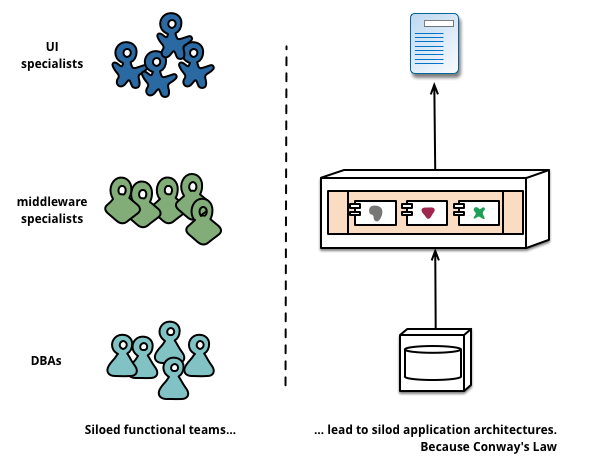
\includegraphics{ConwaysLaw}
	\centering
\end{figure}
The Microservice approach changes the view of division with development teams. This approach involves organising teams around developing services based on the businesses capabilities – accounts service, basket service, payment service, catalogue service, car insurance service etc. These services implement the software needed for that business area: UI, storage, external collaborations etc. The teams become cross-functional consequently, including the full range of skills required for development: database, project management, UI etc. As described by Martin Fowler \cite{MartinFowlersite} in figure \ref{fig:busCapa}. 
\begin{figure}[h]
	\caption{Built around Business Capabilities}
	\label{fig:busCapa}
	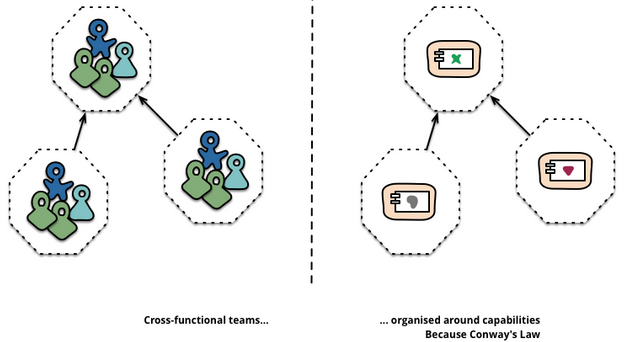
\includegraphics{ConwaysLawOpposite}
	\centering
\end{figure}

\subsubsection{Services are fine-grained Interfaces}
Small, performing only one function – each service is designed to have only one responsibility, perform a single functionality of the business. This single responsibility principle also encompasses the database in use. Instead of having a single database used in a monolithic system, each Microservice can have its own database to store the data. This is a change from the Monolithic style where a single database would be used to store the systems data. Although, several Microservice could access the same database, again, depending on the context of the software system.

The services are described as “fine grained” referring to the granularity of the Services themselves. The actual size of the service varies depending on the context of the business. How small or fine grained a service must be is open for discussion. A general agreement is that the codebase of the service should be manageable by a small team of people.  For example, Amazon \cite{HoffAmazonArchi} has coined the phrase “the two-pizza teams” – each team numbers around 8-10 people. The number you can feed off two pizzas . Meaning the code base for the Microservice would only be “big enough” for this number of people to handle. Similarly, Jon Eaves, of RealEstate.com.au, characterizes a Microservice as something that could be rewritten in two weeks as stated by Sam Newman \cite{NewmanMSA}).

Zimmerman \cite{Zimmermann2017} reinforces this definition of: "Services that can be deployed,c hanged, substituted and scaled independently of each other" and states fine-grained services as one of the seven common tenets cited in introductory literature and case studies on Microservices.

\subsubsection{Services are designed to fail}
By creating services as components, applications that use these services need to be designed so they tolerate any failure of services \cite{MartinFowlersite}. This introduces another layer of complexity when designing microservices. Services can and will fail, but the effect on users must be limited.

It is important to detect failures as quickly as possible and restore them, automatically if possible. The MSA puts emphasis on real-time monitoring of the application; checking architectural (database requests per second) and business relevant (orders per minute received etc) metrics \cite{MartinFowlersite}. Monitoring can lead to early warning signs of a failure, that will allow development teams to proactively investigate.

This will likely lead to complex, and expensive, monitoring systems in place – The Microservice teams need to know which services, running in different processes, have failed. This is generally achieved by having separate, sophisticated monitors and logging set-ups for each service available. Monitoring such things as: up/down status and operational/business relevant metrics \cite{MartinFowlersite}.

Famously, Netflix created a set of tools dubbed the “Simian army” that were developed solely to generate various kinds of failures and test the robustness of their system. \cite{SimianArmy}. 

\subsubsection{Microservice Architecture has a natural modular Structure}
As described previously, each service is a component of the system and, thus, enforces a modular structure where each service is seen as a module. This implementation of Modular Programming \cite{TechopediaModular} encompasses many of its benefits:

Each service can be used many times by many users. This benefit is adhered too as the code written, for each service, is not repeated. Only the service needed is called upon, through events etc., and executes the required task(s).

This modularity allows for each service to be used in conjunction with other applications. As service independence is a requirement of the MSA, the services can be used in the creation of multiple applications.

A disadvantage with the modular structure of the Microservice architecture occurs in the debugging of the system.  

\subsubsection{Encourages Infrastructure Automation and Testing}
As different businesses have different needs, the number of microservices developed can differ greatly. As the Microservice architecture adheres to the distributed systems model; microservices will be deployable on multiple servers/machines and it can become difficult, almost impossible, to develop, test, deploy, monitor each Microservice manually. Regardless of the size \& number of software development teams. The answer to this is to introduce automation. 

The development of the Cloud and Amazon Web Services (AWS) have reduced the operational complexity of building, deploying and operating microservices \cite{MartinFowlersite}. These infrastructure automation techniques have evolved extensively over the last few years.

Current systems built using microservices are development by teams with extensive Continuous delivery (discussed later) experience \cite{MartinFowlersite}. Software built using this principle make extensive use of the above infrastructure automation techniques. This helps to streamline and automate the testing of builds.  See figure \ref{fig:autoTestDeploy}.
\begin{figure}[h]
	\caption{Automated testing to deployment}
	\label{fig:autoTestDeploy}
	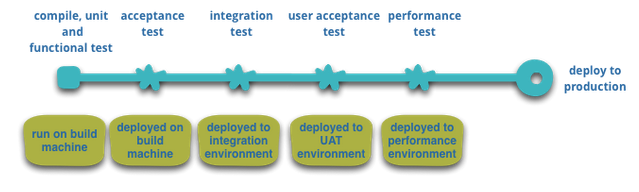
\includegraphics{AutomatedTestingDeployment}
	\centering
\end{figure}
Current systems built using microservices are development by teams with extensive Continuous delivery (discussed later) experience (Fowler, 2014). Software built using this principle make extensive use of the above infrastructure automation techniques. This helps to streamline and automate the testing of builds.

Testing and deployment automation brings several advantages:
\begin{itemize}
	\item allows teams to choose when they want to deploy the microservices they are in control of. Potentially deploying new builds multiple times in a short period of time.
	\item Newly developed/updated features are in the hands of customers faster
	\item Allows for frequent testing of new features
	\item Teams can experiment new processes, algorithms etc. Lokesh Gupta \cite{GuptaMSA} describes this as Enterprises being given the ability to experiment and fail fast.
\end{itemize}
But there are disadvantages.
A potential risk to continuous deployment/integration is “moving fast and breaking things” \cite{HunterAdvMSA}. If backward compatibility is not diligently adhered too, for versioning deployments, a change can be released that results in the Microservice breaking and affecting consumers.
\subsubsection{Introduces the concept of you built it you own it}
Depending on the scale of the services provided by companies, there can be hundreds of microservices within a company’s software system structure. For example, Amazon, one of the first companies to embrace MSA, has over 150 services and can up to 100 of these services to build a single web page \cite{HoffAmazonArchi}. Services include: Search, register, account, catalogue, refine, recommendations etc.

